% Documentation of the AnnotaStruct sensor

\subsubsection{\texttt{Sensor.AnnotaStruct}}
\label{annotastruct}
\paragraph{Description}

The sensor allows to seamlessly modify \EuGene\ underlying graph
weighting using a small langage that can directly modify the weights
of signals and contents edges in the graph. The plugin offers both
high-level entries and low-level entries in either a sloppy GFF-like
format or a strict GFF3-compliant format.

The high-level entries allow to take into account information on:
\begin{itemize}
\item \textbf{transcribed sequences} (involving exons, introns, UTR,
  transcription start and transcription stop and splice sites) that
  may come from alignment of transcribed sequences (using spliced
  alignment algorithms such as sim4 or PASA).
\item \textbf{CDS} (involving exons, introns, translation start,
  translation stop and splice sites) that may come from other gene
  predictors that may predict CDS (either \emph{ab initio} or homology based
  predictors).
\item \textbf{ncRNA} (involving non protein coding RNA region, ncRNA transcription start and ncRNA transcription stop).
\end{itemize}
The high-level entries are actually automatically expanded in
elementary (low-level) information as the plugin reads the data. The
way the expansion takes place is user-controllable through parameters.

Compared to the \texttt{Est} plugin, there is no data filtering
performed here which means that the plugin should rather be used on
consistent and fairly reliable data (eg. on existing gene predictions,
cDNA or EST cluster alignements rather than simple EST alignments that
would be better handled using the \texttt{Est} plugin).

The low-level entries allow to directly modify every edge of the
underlying prediction graph of \EuGene\ as the (now obsolete)
\texttt{User} plugin allowed. The weights of all signals edges
(transcription start and stop, translation start and stop, splice
sites, insertions and deletions, ncRNA transcription start and stop) 
and contents edges (exons, introns,
UTR, UTR introns, intergenic regions and ncRNA) can be directly modified
using this plugin.

To activate the sensor, put the number of AnnotaStruct instances you want to create to the parameter
\texttt{Sensor.AnnotaStruct.use} in the parameter file.

Here is an example of AnnotaStruct parameters definition :
\begin{Verbatim}[fontsize=\small]
AnnotaStruct.FileExtension[0]    gff
AnnotaStruct.TranscriptFeature[0]  mRNA
AnnotaStruct.Exon*[0]            1
AnnotaStruct.Intron*[0]          2
AnnotaStruct.CDS*[0]             3
AnnotaStruct.npcRNA*[0]          2
AnnotaStruct.Intergenic*[0]      0
AnnotaStruct.StartType[0]        p 
AnnotaStruct.Start*[0]           0.1
AnnotaStruct.StopType[0]         p 
AnnotaStruct.Stop*[0]            0.1
AnnotaStruct.AccType[0]          p 
AnnotaStruct.Acc*[0]             0.1
AnnotaStruct.DonType[0]          p 
AnnotaStruct.Don*[0]             0.1
AnnotaStruct.TrStartType[0]      p 
AnnotaStruct.TrStart*[0]         0.1
AnnotaStruct.TrStopType[0]       p 
AnnotaStruct.TrStop*[0]          0.1
AnnotaStruct.TrStartNpcType[0]   p
AnnotaStruct.TrStartNpc*[0]      0.1
AnnotaStruct.TrStopNpcType[0]    p
AnnotaStruct.TrStopNpc*[0]       0.1

Sensor.AnnotaStruct.use       1         # Use one AnnotaStruct sensor instance
Sensor.AnnotaStruct          1         # Sensor priority
\end{Verbatim}

\paragraph{Native GGF-like input files format}

The plugin reads a GFF format file. Each line in this file forms an
elementary information which is directly interpreted by the plugin
independently of other lines. A GFF line is formed by a sequence of
separated fields: sequence name, source, feature, start, end, score,
strand and frame. The sequence name and source fields are ignored by
the plugin and can be set to user informative values.

Each line may either represent a high-level or a low-level
information.  Low-level informations use specific features for
specifying which signals and contents edges should be modified. For
signals, the following features are recognized:
\begin{itemize}
\item \texttt{trStart}: for transcription starts.
\item \texttt{trStop}: for transcription stops.
\item \texttt{start}: for translation starts (ATG).
\item \texttt{stop}: for translation stops.
\item \texttt{acc}: for acceptor splice sites.
\item \texttt{don}: for donor splice sites.
\item \texttt{ins}: for insertion (frameshift).
\item \texttt{del}: for deletion (frameshift).
\item \texttt{trStartNpc}: for ncRNA transcription starts.
\item \texttt{trStopNpc}: for ncRNA transcription stops.
\end{itemize}
In this case, the start and the strand field are used to indicate the
signal position. The score field is used to indicate the weight that
will be used to modify the existing weight. It is either a floating
point value between \texttt{-1e999} and \texttt{1e999} (that match
$-\infty$ and $\infty$ respectively in the format used) or a floating point
between $0.0$ and $1.0$ preceded by the letter $p$ (like probability).

\begin{enumerate}
\item In the first case, the score indicated is directly added to the
  weight of the signal edge (that corresponds to the fact that the
  signal is used). The other signal edge is unmodified.
\item In the second case, the score $s$ that appears after the $p$ is
  treated as a (conditional) probability. The edge that corresponds to
  the fact that the signal is used receive a weight $\log(s)$ and the
  other edge $\log(1-p)$.
\end{enumerate}

For contents edges, the following features are recognized:
\begin{itemize}
\item \texttt{interg}: for non transcribed regions
\item \texttt{exon}: for coding exons.
\item \texttt{intron}: for introns separating coding exons.
\item \texttt{utr5}: for 5' UTR (untranslated terminal regions).
\item \texttt{utr3}: for 3' UTR.
\item \texttt{utr}: for both 5' or 3' UTR.
\item \texttt{intronutr}: for UTR introns.
\item \texttt{ncrna}: for non protein coding RNA.
\end{itemize}
The start and end fields together with the strand field delimit the
region considered. All corresponding contents edges will be modified
by the weight indicated in the score field.



High-level information may either be used to express knowledge about
potential \emph{transcribed sequences} or potential \emph{coding
  sequences}. For information about CDS regions, the following
features may be used:
\begin{itemize}
\item \texttt{E.Init}: for an initial exon, this will automatically
  expand in the weight modification of a translation start and a donor
  site at the corresponding extremities on the indicated strand (using
  parameters \texttt{AnnotaStruct.Start*} and
  \texttt{AnnotaStruct.Don*} respectively as weights) and the contents
  modification for the exon in the corresponding frame and strand
  (using the score indicated in the \texttt{AnnotaStruct.CDS*}
  parameter).
\item \texttt{E.Intr}: for an intermediary exon, this will
  automatically expand in the weight modification of a donor and an
  acceptor site at the corresponding extremities on the indicated
  strand (using parameters \texttt{AnnotaStruct.Don*} and
  \texttt{AnnotaStruct.Acc*} respectively as weights) and the contents
  modification for the exon in the corresponding frame and strand
  (using the score indicated in the \texttt{AnnotaStruct.CDS*}
  parameter).
\item \texttt{E.Term}: for a terminal exon, this will automatically
  expand in the weight modification of an acceptor and a stop signal
  at the corresponding extremities on the indicated strand (using
  parameters \texttt{AnnotaStruct.Acc*} and \texttt{AnnotaStruct.Stop*}
  respectively as weights) and the contents modification for the exon
  in the corresponding frame and strand (using the score indicated in
  the \texttt{AnnotaStruct.CDS*} parameter).
\item \texttt{E.Sngl}: for a single exon gene, this will automatically
  expand in the weight modification of a translation start and stop
  signal at the corresponding extremities on the indicated strand
  (using parameters \texttt{AnnotaStruct.Start*} and
  \texttt{AnnotaStruct.Stop*} respectively as weights) and the
  contents modification for the exon in the corresponding frame and
  strand (using the score indicated in the \texttt{AnnotaStruct.CDS*}
  parameter).
\item \texttt{UTR5}, \texttt{UTR3}, \texttt{UTR}: although not part of
  the CDS, some gene predictors may predict UTR (non coding part of
  exons). These 3 features allow to inject this information by
  respectively reweighting a transcription start, stop or both using
  the corresponding \texttt{AnnotaStruct.TrStart*},
  \texttt{Annota\-Struct.TrStop*} parameters and then by reweighting the
  UTR5, UTR3 or both contents edges (using the
  \texttt{AnnotaStruct.CDS*} parameter).
\item \texttt{Intron}: equivalent to \texttt{intron} except that the
  weight used comes from the \texttt{AnnotaStruct.CDS*} parameter). 
\end{itemize}

For information about transcribed sequences, the following features
are recognized:
\begin{itemize}
\item \texttt{E.Any}: any exon in the biological sense \textit{i.e.}
  either an exon or a UTR in the \EuGene\ sense. Frame is typically
  unknown (in this case, all coding frame in the indicated strand are
  considered). The corresponding contents region are modified
  accordingly to the \texttt{AnnotaStruct.Exon*} parameter.
\item \texttt{E.First}: the first biological exon (containing UTR and
  possibly part of CDS too). A transcription start signal is weighted
  according to the \texttt{AnnotaStruct.TrStart*} parameter value. The
  UTR5 and coding exon contents edges are reweighted according to the
  \texttt{AnnotaStruct.Exon*} parameter value.
\item \texttt{E.Last}: the last biological exon. A transcription stop
  signal is weighted according to the \texttt{Annota\-Struct.TrStop*}
  parameters value. The UTR3 and coding exon contents edge are
  reweighted according to the \texttt{AnnotaStruct.Exon*} parameter
  value.
\item \texttt{E.Extreme}: used for a biological exon on the extremity
  (either first or last).  A transcription start and stop are
  generated at each respective extremities according to the
  \texttt{AnnotaStruct.trStart*} and \texttt{AnnotaStruct.trStop*}
  parameter values. The UTR5, UTR3 and coding exon contents edges are
  reweighted according to the \texttt{AnnotaStruct.Exon*} parameter
  value.
\item \texttt{ncRNA}: a non protein coding RNA (at the moment, EuGene doesn't 
predicted ncRNA intron). A non protein coding transcription start and stop are
  generated at each respective extremities according to the
  \texttt{AnnotaStruct.trStartNpc*} and \texttt{AnnotaStruct.trStopNpc*}
  parameter values. The ncRNA content edge is
  reweighted according to the \texttt{AnnotaStruct.npcRNA*} parameter
  value.
\item \texttt{Intron.Any}: ?
\end{itemize}


Here is a high-level CDS based example:
\begin{Verbatim}[fontsize=\small]
ATSYNO FGENESH E.Init  3 33 0 + 3
ATSYNO FGENESH E.Term 45 75 0 + 3
\end{Verbatim}

\paragraph{Gff3 input files format}

The gff3 input mode is activated by setting the value \texttt{GFF3}
for the parameter \texttt{AnnotaStruct.format} in the parameter file.
The plugin reads its informations from a file named with the sequence
name and an extension \texttt{AnnotaStruct.FileExtension} followed by
\texttt{.gff3} In gff3 mode, you can't describe feature level as in
natif mode.

If you want to read scores or probabilities from file you have to set
parameters score to "i" (for "inline") in the parameter file. Content data will
always be interpreted as score.
\begin{Verbatim}[fontsize=\small]
AnnotaStruct.Exon*            i  # interpreted as score
AnnotaStruct.Intron*          i  # interpreted as score
AnnotaStruct.CDS*             i  # interpreted as score
AnnotaStruct.npcRNA*          i  # interpreted as score
AnnotaStruct.Intergenic*      i	 # interpreted as score
AnnotaStruct.StartType        p  # p: probability  s: score 
AnnotaStruct.Start*           i
AnnotaStruct.StopType         p  # p: probability  s: score 
AnnotaStruct.Stop*            i
AnnotaStruct.AccType          p  # p: probability  s: score 
AnnotaStruct.Acc*             i
AnnotaStruct.DonType          p  # p: probability  s: score 
AnnotaStruct.Don*             i
AnnotaStruct.TrStartType      p  # p: probability  s: score 
AnnotaStruct.TrStart*         i
AnnotaStruct.TrStopType       p  # p: probability  s: score 
AnnotaStruct.TrStop*          i
AnnotaStruct.TrStartNpcType   p # p: probability  s: score 
AnnotaStruct.TrStartNpc*      i
AnnotaStruct.TrStopNpcType    p # p: probability  s: score   
AnnotaStruct.TrStopNpc*       i
\end{Verbatim}

Here is the correspondance beetween GFF native AnnotaStruct features
and GFF3 features. A direct translation between the two formats is not
always possible (for example, low-level content information cannot be
given directly in GFF3, but can be indirectly achieved by setting
signal at zero, and using the transcribed sequence feature).

Each GFF feature is translated in a GFF3 feature (column 3 in the GFF3 file). 
Some may require an additional ontology term (specified in the column 9 with the key Ontology\_term). 
The expected value in the column 3 and if an Ontology\_term is required, the expected value in the column 9, are given below.

Low-level information:
\begin{itemize}
\item \texttt{trStart}: 	SO:0000315 (or TSS)
\item \texttt{trStop}: 	SO:0000616 (or transcription\_end\_site)
\item \texttt{start}: 	SO:0000318 (or start\_codon).
\item \texttt{stop}: 	SO:0000319 (or stop\_codon)
\item \texttt{acc}: 	SO:0000164 (or three\_prime\_cis\_splice\_site)
\item \texttt{don}: 	SO:0000163 (or five\_prime\_cis\_splice\_site)
\item \texttt{ins}: 	SO:0000366 (or insertion\_site)
\item \texttt{del}: 	SO:0000687 (or deletion\_junction)
\item \texttt{trStartNpc} and \texttt{trStopNpc} : no corresponding feature
\end{itemize}

High-level information:

Translated regions information
\begin{itemize}
\item \texttt{E.Init}: CDS (or SO:0000316)                + Ontology\_term=SO:0000196 (five\_prime\_coding\_exon\_region)
\item \texttt{E.Intr}: CDS (or SO:0000316)                + Ontology\_term=SO:0000004 (interior\_coding\_exon)
\item \texttt{E.Term}: CDS (or SO:0000316)                + Ontology\_term=SO:0000197 (three\_prime\_coding\_exon\_region)
\item \texttt{E.Sngl}: CDS (or SO:0000316)                + Ontology\_term=SO:0005845 (single\_exon)
\item \texttt{UTR5}:   five\_prime\_UTR  (or SO:0000204)
\item \texttt{UTR3}:   three\_prime\_UTR (or SO:0000205)
\item \texttt{UTR}:    UTR (or SO:0000203)
\item \texttt{Intron}: intron (or SO:0000188)             + Ontology\_term=SO:0000191 (interior\_intron)
\end{itemize}

Transcribed region information
\begin{itemize}
\item \texttt{E.Any}: 		exon (or SO:0000147)
\item \texttt{E.First}: 	exon (or SO:0000147)	  + Ontology\_term=SO:0000200 (five\_prime\_coding\_exon)
\item \texttt{E.Last}: 		exon (or SO:0000147)	  + Ontology\_term=SO:0000202 (three\_prime\_coding\_exon)
\item \texttt{E.Extreme}: 	exon (or SO:0000147)	  + Ontology\_term=SO:0000200,SO:0000202
\item \texttt{Intron.Any}: 	intron (or SO:0000188)
\item \texttt{transcript}: transcript\_region (or SO:0000833)
\item \texttt{ncRNA}: 	        ncRNA (or SO:0000655 or other SO terms derived from ncRNA, for instance rRNA (SO:0000252) or tRNA (SO:0000253). 
See  \texttt{http://www.sequenceontology.org/wiki/index.php/} \texttt{Category:SO:0000655\_!\_ncRNA} for details.
\end{itemize}

Intergenic information
\begin{itemize}
\item \texttt{interg}: intergenic\_region (or SO:0000605)
\end{itemize}



\begin{figure}[h]
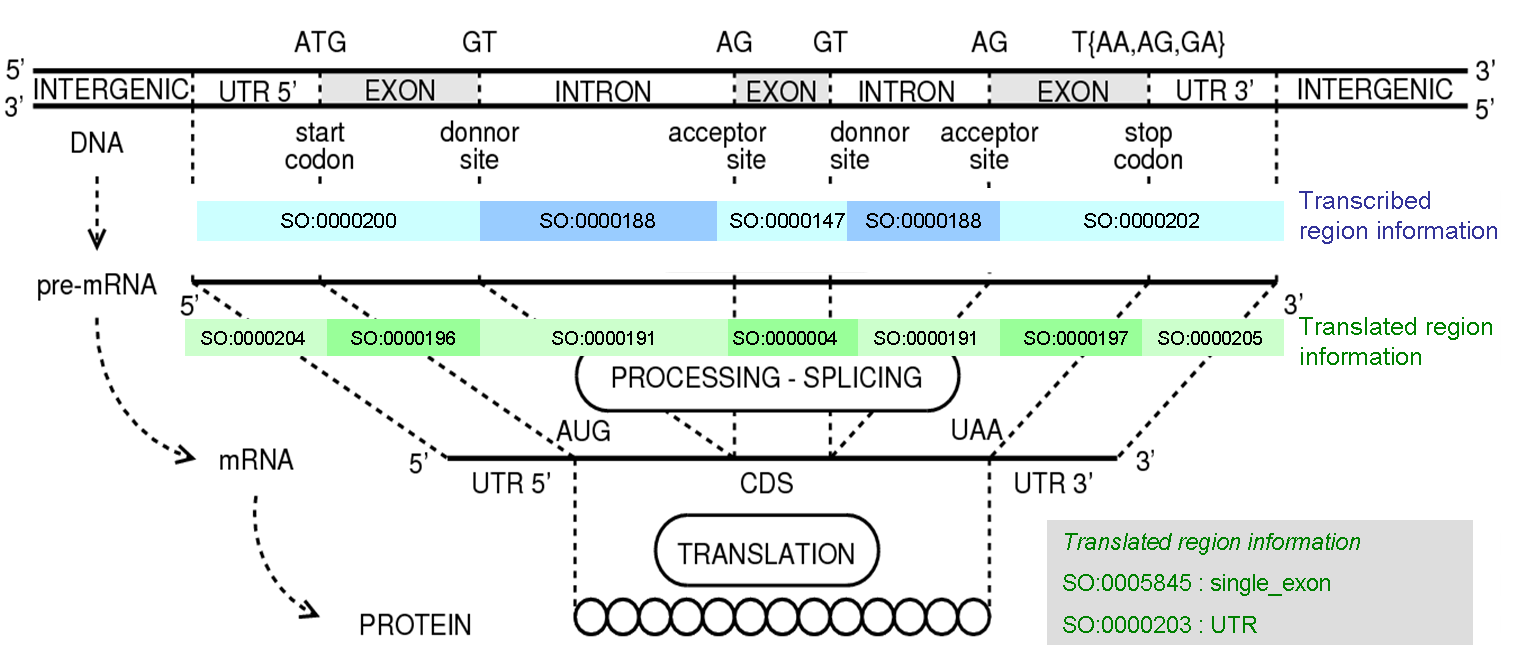
\includegraphics[width=17cm]{SO.png} 
\end{figure}

Here an extract of : seq14ac002535g4g5.tfa.gff.gff3
\begin{Verbatim}[fontsize=\tiny]
seq25	EuGene	five_prime_UTR	1	2787	0	+	.	ID=five_prime_UTR:seq25.0;
seq25	EuGene	CDS	2788	2836	0	+	0	ID=CDS:seq25.1;Ontology_term=SO:0000196
seq25	EuGene	CDS	8356	8471	0	+	2	ID=CDS:seq25.2;Ontology_term=SO:0000004
seq25	EuGene	CDS	8576	8667	0	+	1	ID=CDS:seq25.3;Ontology_term=SO:0000004
seq25	EuGene	CDS	9006	9061	0	+	0	ID=CDS:seq25.4;Ontology_term=SO:0000004
seq25	EuGene	CDS	9567	9655	0	+	1	ID=CDS:seq25.5;Ontology_term=SO:0000004
seq25	EuGene	CDS	10520	10535	0	+	1	ID=CDS:seq25.6;Ontology_term=SO:0000004
seq25	EuGene	CDS	10896	11134	0	+	1	ID=CDS:seq25.7;Ontology_term=SO:0000004
seq25	EuGene	CDS	11544	12005	0	+	2	ID=CDS:seq25.8;Ontology_term=SO:0000004
seq25	EuGene	CDS	12088	12900	0	+	0	ID=CDS:seq25.9;Ontology_term=SO:0000197
seq25	EuGene	three_prime_UTR	12901	14900	0	+	.	ID=three_prime_UTR:seq25.10;
\end{Verbatim}

For complete gene, ontology terms for CDS can be added on the fly by the plugin if the GFF3 includes Parent information to a transcript level feature. This feature is typically called "mRNA" or "transcript" in gene finders GFF3 output.
If the \texttt{AnnotaStruct.TranscriptFeature} parameter is set accordingly, then the plugin will identify first, internal, terminal and single exon assuming the CDS features are in increasing position order.

\paragraph{Filtering input information}

No filtering beside syntax checking.

\paragraph{Integration of information}

The underlying graph edges are directly modified as indicated. 

\paragraph{Post analyse}

No post analyse.

\paragraph{Graph}

No plotting.




